\documentclass[xcolor={x11names, rgb, usenames, dvipsnames}]{beamer}
% Beamer loads xcolor by default. Do not load it a second time using \usepackage

\usepackage[francais, english]{babel}
\usepackage[T1]{fontenc}
\usepackage[utf8]{inputenc}
\usepackage{pgfplots}
\pgfplotsset{compat=newest}
\usepackage{graphicx}
\usepackage{hyperref}
\usepackage{amsmath}


%\usetheme{Warsaw}
% \usetheme{Boadilla}
% \usetheme{Antibes}
\usetheme{CambridgeUS}
\usecolortheme{dolphin}
% \usetheme{Berlin}
% \usetheme{Madrid}
% \setbeamertemplate{footline}[frame number]

\author{Quentin Delhaye}
\title[INFOH414 -- Swarm Intelligence]{INFOH414 -- Swarm Intelligence}
\subtitle{Collective Decision Making with Homogeneous Agents}
\institute[ULB]{Université Libre de Bruxelles}
\date{September 4th, 2015}

\begin{document}

\begin{frame}
\titlepage
\end{frame}

\begin{frame}
	%\tableofcontents[hideallsubsections]
	\tableofcontents
\end{frame}


%%%%%%%%%%%%%%%%%%%%%%%%%%%%%%%%%%%%%%%%%%%%
\section{Introduction}
%%%%%%%%%%%%%%%%%%%%%%%%%%%%%%%%%%%%%%%%%%%%

\begin{frame}
\frametitle{Introduction}
\begin{itemize}
	\item Use LEDs to encode room quality
	\item Remember only the last room
	\item Best room sensed overwrites the last room quality
	\item Random movement based on collision avoidance
\end{itemize}
\end{frame}



%%%%%%%%%%%%%%%%%%%%%%%%%%%%%%%%%%%%%%%%%%%%
\section{Idea}
%%%%%%%%%%%%%%%%%%%%%%%%%%%%%%%%%%%%%%%%%%%%

\begin{frame}
\frametitle{Idea}
\begin{itemize}
	\item Go to closest room
	\item Get quality
	\item Go back to central room
	\item Broadcast last room quality and sense other's
	\item Move toward best room sensed
\end{itemize}
\end{frame}



%%%%%%%%%%%%%%%%%%%%%%%%%%%%%%%%%%%%%%%%%%%%
\section{Analysis}
%%%%%%%%%%%%%%%%%%%%%%%%%%%%%%%%%%%%%%%%%%%%

\begin{frame}
\frametitle{Repartition}
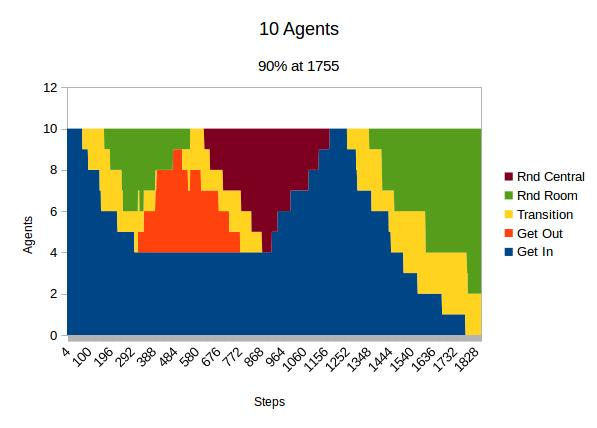
\includegraphics[height=\textheight]{agents_10}
\end{frame}

\begin{frame}
\frametitle{Repartition}
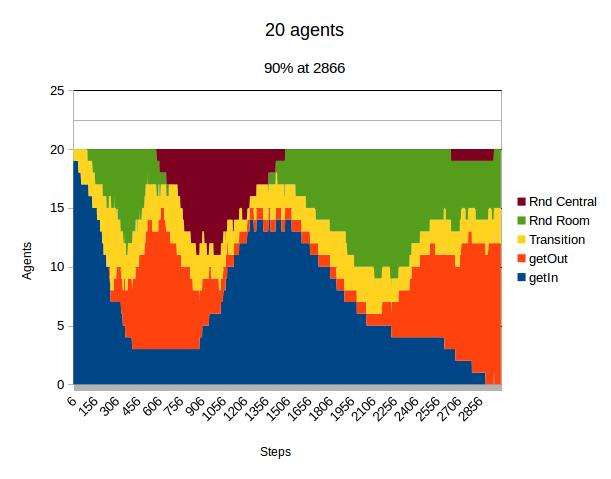
\includegraphics[height=\textheight]{agents_20}
\end{frame}

\begin{frame}
\frametitle{Repartition}
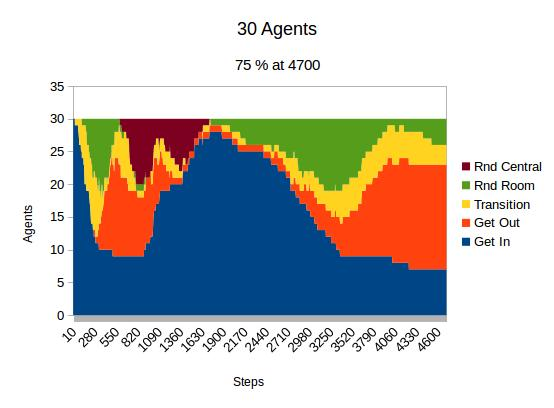
\includegraphics[height=\textheight]{agents_30}
\end{frame}

% \begin{frame}

% \end{frame}

% \begin{frame}

% \end{frame}

% \begin{frame}

% \end{frame}






%%%%%%%%%%%%%%%%%%%%%%%%%%%%%%%%%%%%%%%%%%%%
\section{Conclusion}
%%%%%%%%%%%%%%%%%%%%%%%%%%%%%%%%%%%%%%%%%%%%
\begin{frame}
\frametitle{Conclusion}
\begin{itemize}
	\item More robots means more congestion
	\item Consider DoL: specialize explorators and quality propagators
	\item Need for interference reduction
	\item Need to stay longer in highest quality room, don't leave if the entrance is saturated
\end{itemize}
\end{frame}
		

\end{document}
